Для установившегося режима фильтрации давление в пласте не меняется. Для псевдо-установившегося режима постоянным остается перепад давления между пластом и забоем. После запуска, остановки или изменения режима работы скважины эти условия не выполняются. Давление в различных точках пласта может меняться по разному. Такой режим называют неустановившимся, а решения его описывающие нестационарными (зависят от времени).

Неустановившиеся решения уравнения фильтрации (transient solutions) представляют значительный практический интерес во многих задачах, включая задачи интерпретации ГДИС. В тоже время они относительно сложны и требуют применения компьютерных алгоритмов. В данном пособие проведение расчетов иллюстрируется с использованием макросов для Excel -- Unifloc VBA.

\subsection{Безразмерные переменные}

Часто для анализа уравнений неустановившейся фильтрации используются безразмерные переменные 

\marginpar{
	\href{https://en.wikipedia.org/wiki/Nondimensionalization}{Обезразмеривание на en.wikipedia.org} 
	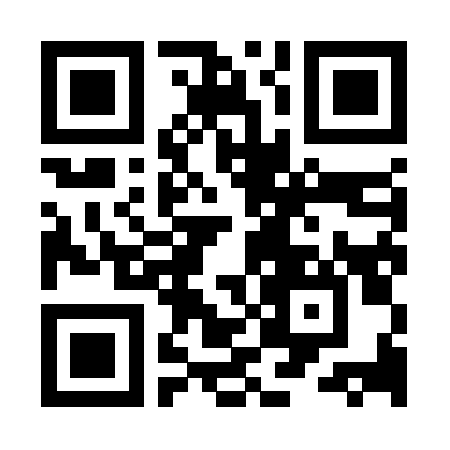
\includegraphics[scale=0.4]{pics/qr_Nondimensionalization.eps} 
}

$$ r_D = \frac{r}{r_w} $$
$$ t_D = \frac{kt}{\varphi \mu c_t r_w^2}$$
$$ p_D = \frac{2 \pi kh}{q_s B \mu} \left( p_i - p_{wf} \right) $$

Здесь использование единицы измерения СИ. 

$q_s$ - дебит скважины на поверхности, приведенный к нормальным условиям м3/с

$\varphi$ - пористость, доли единиц

$\mu$ - вязкость нефти в пласте, Па с

$B$ - объемный коэффициент нефти, м3/м3

$p_i$ - начальное давление в пласте, Па

$p_{wf}$ - давление забойное, Па

$c_t$ - общая сжимаемость системы в пласте, 1/Па

\

Использование безразмерных переменных позволяет упростить уравнение фильтрации, которое примет вид

$$ \frac{\partial p_D}{ \partial t_D} = \frac{1}{r_D} \frac{ \partial{ \left( r_D \dfrac{\partial p_D}{ \partial r_D} \right) } }{ \partial{r_D} } $$

Решение этого уравнения - функция безразмерного давления от безразмерных времени и расстояния $p_D(r_D, t_D) $

Для практических расчетов удобнее бывает использовать безразмерные переменные полученные для практических метрических единиц измерения. 
$$ r_D = \frac{r}{r_w} $$
$$ t_D = \frac{0.00036 kt}{\varphi \mu c_t r_w^2}$$
$$ p_D = \frac{kh}{ 18.41 q_s B \mu} \left( p_i - p_{wf} \right) $$

Здесь использование единицы измерения СИ. 

$q_s$ - дебит скважины на поверхности, приведенный к нормальным условиям м3/сут

$\varphi$ - пористость, доли единиц

$\mu$ - вязкость нефти в пласте, сП

$B$ - объемный коэффициент нефти, м3/м3

$p_i$ - начальное давление в пласте, атм

$p_{wf}$ - давление забойное, атм

$c_t$ - общая сжимаемость системы в пласте, 1/атм

\

Дополнительно можно ввести безразмерный коэффициент влияния ствола скважины
$$ C_D = \frac{0.159}{ h \varphi \mu c_t r_w^2 } C_s $$

\subsubsection{Расчет безразмерных переменных в Unifloc VBA}

Несмотря на простоту определений безразмерных переменных их часто приходится применять при проведении расчетов. Поэтому в надстройке Unifloc VBA реализован набор функций расчета безразмерных переменных.

Эти функции начинаются с префикса  transient\_def.

\begin{verbatim}
	transient_def_cd
	transient_def_cs_1atm
	transient_def_td
	transient_def_t_day
	transient_def_pd
	transient_def_pwf_atma
\end{verbatim}	

Описания функций и из аргументов можно найти в руководстве пользователя  Unifloc VBA

\subsection{Решение линейного стока}

Для решения уравнения фильтрации - линейного дифференциального уравнения в частных производных второго порядка необходимо задать начальные и граничные условия. 

Самое простое решение можно получить для случая вертикальной скважины бесконечно малого радиуса запускающейся с постоянным дебитом. Условия соответствующие этому случаю можно выразить следующим образом:

\begin{itemize}
	\item Начальное условие. До запуска скважины в момент времени  $t_D = 0$ давление в пласте равно начальному во всех точках $p=p_i$
	$$ t_D < 0, p_D = 0 $$ 
	\item Граничное условие на скважине.  Условие постоянства дебита на скважине можно трансформировать в граничное условие опираясь на закон Дарси.
	$$ \lim_{r_D \to 0} {r_D \frac{\partial p_D}{\partial r_D}} = -1$$
	\item Граничное условие на бесконечном расстоянии от скважины. Давление в пласте на бесконечно большом расстоянии от скважины равно начальному.
	$$ r_D = \infty, p_D = 0$$
\end{itemize}

\begin{wrapfigure}{r}{0.5\textwidth}
	%\begin{figure}[h!]
	\begin{center}
		\begin{tikzpicture}
			\begin{axis}
				[axis lines = left,
				 width = 0.98\textwidth,
				%xlabel=$x$,
				%ylabel={$Ei_1(x)$},
				]
				\addplot gnuplot[no markers, samples=100, domain = 0:10]{expint(1,x)};
				\addlegendentry{$Ei_1(x)$}
			\end{axis}
		\end{tikzpicture}
		\caption{График функции интегральной экспоненты $Ei_1(x)$.}
		\label{ris:ei1}
	\end{center}
	%\end{figure}
\end{wrapfigure}



В этом случае решение может быть выражено через функцию интегральной экспоненты 
$$ p_D(r_D,t_D) = - \frac{1}{2} Ei \left(- \dfrac{ r_D^2}{4t_d} \right)$$

где $-Ei(-x)$ - интегральная показательная функция.

$$Ei(x)=-\int\limits_{x}^{\infty}\frac{e^{-t}}{t}\,\mathrm dt$$

\marginpar{
	\href{https://www.wolframalpha.com/input/?i=Ei\%28x\%29}{$Ei(x)$ на Wolfram Alpha} 
	
\includegraphics[scale=0.4]{pics/qr_ei_wolfram.eps} 
	}

Часто для проведения расчетов, особенно с использованием компьютерных библиотеке расчетов, бывает удобнее пользоваться модифицированной интегральной показательной функцией $Ei_1(x)$ или $E_1(x)$ или $Ei_n(x)$ при $n=1$.
 $$Ei_n(x) = \int\limits_{1}^{\infty}\frac{e^{-tx}}{t^n}\,\mathrm dt $$

График интегральной показательной функции $Ei_1(x)$ приведен на рисунке \ref{ris:ei1}.
Для вещественных положительных $x\in\mathbb R, x>0$ верно $E_1(x) = - Ei( -x)$

Функцию интегральной экспоненты можно представить в виде ряда. 

$$Ei(x)=-\int\limits_{x}^{\infty}\frac{e^{-t}}{t}\,\mathrm dt=\gamma+\operatorname{ln}|-x|+\sum\limits_{n\ge1}\frac{{-x}^n}{n!\cdot n}, \;  x\in\mathbb R,\;$$

\begin{wrapfigure}{r}{0.5\textwidth}
	%\begin{figure}[h!]
	\begin{center}
		\begin{tikzpicture}
			\begin{axis}
				[axis lines = left,
				width = 0.98\textwidth,
				%xlabel=$x$,
				%ylabel={$f(x)$},
				]
				\addplot gnuplot[no markers, samples=100, domain = 0:2]{expint(1,x)};
				\addlegendentry{$Ei_1(x)$}
				\addplot gnuplot[no markers, samples=100, domain = 0:2]{-log(x)-0.5772};
				\addlegendentry{$ln(x)$}
			\end{axis}
		\end{tikzpicture}
		\caption{Сравнение функций интегральной экспоненты $E_1(x)$ и $ln(x)$.}
		\label{ris:ei2}
	\end{center}
	%\end{figure}
\end{wrapfigure}

Из приведенного выражения можно сделать выводы, что для маленьких значений аргумента  функция интегральной экспоненты $E_1(x)$ может быть аппроксимирована логарифмической зависимостью. 

$$E_1(x) = -ln(x) - \gamma $$

График сравнения функций $E_1(x)$ и $ln(x)$ показан на рисунке \ref{ris:ei2}. Видно, что хорошей аппроксимация будет только для маленьких значений аргумента $x < 0.01$. Но для решения уравнения фильтрации именно эта зона представляет наибольший интерес.

%\begin{wrapfigure}{r}{0.5\textwidth}
\begin{figure}[h!]
	\begin{center}
		\begin{tikzpicture}
			\begin{axis}
				[axis lines = left,
				width = 0.98\textwidth,
				xlabel=$x$,
				ylabel={$f(x)$},
				xmode=log,
				log ticks with fixed point,
				]
				\addplot gnuplot[no markers, samples=100, domain = 0.00001:20 ]{expint(1,x)};
				\addlegendentry{$Ei_1(x)$}
				\addplot gnuplot[no markers, samples=100, domain = 0.00001:20]{-log(x)-0.5772};
				\addlegendentry{$ln(x)$}
			\end{axis}
		\end{tikzpicture}
		\caption{Сравнение функций интегральной экспоненты $E_1(x)$ и $ln(x)$ в логарифмическом масштабе.Можно оценить диапазон применимости логарифмической аппроксимации.}
		\label{ris:ei3}
	\end{center}
\end{figure}
%\end{wrapfigure}

Представление интегральной экспоненты в виде логарифмической аппроксимации удобно на практике, так как логарифм легче вычислять. В большинстве языков программирования и инструментов для проведения расчетов расчет логарифма реализован по умолчанию. А для расчета интегральной экспоненты, часто приходится предпринимать дополнительные шаги.

Решение уравнения фильтрации для линейного стока с учетом логарифмической аппроксимации можно представить в виде 
$$ p_D(r_D,t_D) = \frac{1}{2} \left( ln \left( \dfrac{ t_D }{r_D^2}  \right) +0.809 \right) $$

при использовании данного уравнения, следует помнить, что приближенное решение применимо при $\dfrac{r_D^2}{4t_D} < 0.01$

Решение линейного стока в размерных переменных
$$ p\left(r,t\right)=p_i-\frac{18.41q_sB\mu}{kh}\left(-\frac{1}{2}Ei\left(-\frac{\varphi\mu c_tr^2}{0.00144kt}\right)\right) $$

Решение с учетом логарифмической аппроксимации в размерных переменных
$$ p\left(r,t\right)=p_i-\frac{9.205q_sB\mu}{kh}\left(ln{\frac{kt}{\varphi\mu c_tr^2}}-7.12\right)$$
верно при 
$$\frac{kt}{\varphi\mu c_tr^2}>70000 $$

Решения приведены для практических метрических единиц измерения, что можно увидеть по размерному коэффициенту. 

Скин фактор и нестационарное решение
$$ P(r, t) = P_{i} - \frac {9.205 {q_s} B\mu }{k h}(\ ln\frac {k t}{ \varphi \mu {c_t} {r^2}} -7.12 + 2S) $$


%\subsubsection{Радиус исследования}
%Надо бы тут описать концепцию радиуса исследований и подходы к его оценке

\subsubsection{Расчет в Unifloc VBA}

Следующие функции реализованы в Unifloc VBA

\begin{verbatim}
	Ei
	E_1
\end{verbatim}	

Описания функций и из аргументов можно найти в руководстве пользователя  Unifloc VBA

\subsection{Решение для конечного радиуса скважины}
Для получения сложных решений уравнения фильтрации часто используется преобразование Лапласа.
\marginpar{
	\href{https://qrgo.page.link/ZUfT2}{преобразование Лапласа} 
	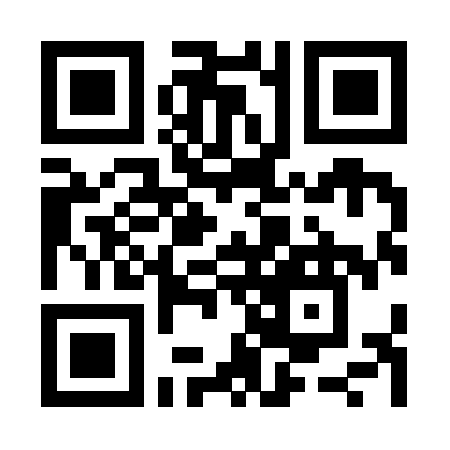
\includegraphics[scale=0.4]{pics/qr_Laplace.eps} 
}

$$ L \left [ f(t) \right] = \tilde{f}(s) = \int_{0}^{\infty}f(t)e^{-st}dt $$

где $s$ параметр пространства Лапласа соответствующий времени

Решение для бесконечно малого радиуса скважины в пространстве Лапласа будет иметь вид

\begin{equation}  \label{eq:laplace_solution_1}
\tilde{p}_D(s) = \frac{1}{s} K_0 \left( r_D \sqrt s  \right) 
\end{equation}

решение для конечного радиуса скважины \cite{Everdingen_1949}

\begin{equation} \label{eq:laplace_solution_2}
	\tilde{p}_D(s) = \frac{K_0 \left( r_D \sqrt{s}  \right) }{ s \sqrt{s} K_1 \left( \sqrt s  \right)  }
\end{equation}

где 

$K_0$, $K_1$ - модифицированные функции Бесселя;

\marginpar{
	\href{https://qrgo.page.link/hkh7x}{модифицированные функции Бесселя} 
	
\includegraphics[scale=0.4]{pics/qr_Bessel.eps} 
}

$s$ - переменная пространства Лапласа;

$\tilde{p}_D(s)$ - изображение функции ${p}_D$ в пространстве Лапласа;

$r_D$ - безразмерный радиус скважины.

\

Перевод решения из пространства Лапласа в обычное пространство не всегда возможен аналитически. В современных условиях перевод делается численно с использованием компьютеров, что позволяет строить и исследования решения уравнения фильтрации при различных условиях. 

Широко распространено применения алгоритма Стефеста для численного обратного преобразования Лапласа. 

\subsubsection{Расчет в Unifloc VBA}

Следующие функции реализованы в Unifloc VBA

\begin{verbatim}
	transient_pd_radial
	transient_pwf_radial_atma
\end{verbatim}	

Описания функций и из аргументов можно найти в руководстве пользователя  Unifloc VBA

\subsection{Учет влияния ствола скважины}
Коэффициент влияния ствола скважины (wellbore storage) определяет сжимаемость жидкости в стволе скважины.


$$ C_s = - \frac{ \Delta V}{ \Delta p} $$

Для фонтанирующей скважины:

Изменение объема жидкости в стволе скважины происходит за счет сжимаемости жидкости:

$$ \Delta V = -c{V_w}{\Delta P} $$

$$ C_s = - \frac{ \Delta V}{ \Delta p} $$

Для фонтанирующей скважины, коэффициент ствола скважины:

$$ C_s =  с {V_w} $$

$ V_w $ - объем жидкости в стволе скважины  [м$^3$]
$c$ - сжимаемость жидкости в стволе скважины [1/атм]

Влияние ствола в механизированной скважине:

$$ C_s = - \frac{ \Delta V}{ \Delta p} $$
$$ {\Delta V} = A_{cas}{\Delta h} $$
$$ {\Delta P} ={ro g}{\Delta h}$$
$$ C_s =  \frac{ A_{cas}}{ \Delta p} $$

$ A_{cas}$ - площадь поперечного сечения затрубного пространства, [м$^2$]


$ {\Delta h}$ - изменение уровня жидкости в затрубном пространстве, [ м ]

Решение уравнения фильтрации с учетом скин-фактор и послепритока
Для решения линейного стока граничное условие соответствующее послепритоку с постоянным $C_s$ можно записать как

$$ \lim_{r_D \to 0} {r_D \frac{\partial p_D}{\partial r_D}} = -1 + \left. C_D \frac{\partial p_D}{\partial t_D} \right|_{t_D=1}$$

Предположим, что у нас имеется решение задачи запуска скважины с постоянным дебитом в прострастве Лапласа без учета скин-фактора и послепритока $\tilde{p}_D^{*}$. Где $s$ параметр пространства Лапласа соответствующий $t_D$.

Например для бесконечного пласта и скважины нулевого радиуса такое решение имеет вид: 

$$\tilde{p}_D^*(s) = \frac{1}{s} K_0 \left( r_D \sqrt s  \right) $$

Тогда решение с учетом скин-фактора и послепритока может быть выражено 

$$\tilde{p}_D(s) = \frac{s \tilde{p}_D^* + S}{s \left( 1+s C_D \left( s \tilde{p}_D^* + S \right)  \right)}   $$



%\subsubsection{Решение для постоянного забойного давления}
%
%\subsubsection{Решение для скважины с ГРП}
%
%Надо привести решение для скважины с ГРП
%
%\subsubsection{Решение для скважины с горизонтальной скважиной}
%
%Надо привести решение для горизонтальной скважины

\subsection{Принцип суперпозиции}

Большинство моделей используемых при интерпретации ГДИС основаны на линеаризованном дифференциальном уравнении в частных производных - уравнении фильтрации (уравнении пьезопроводности или диффузии).

$$ \frac{\partial ^2 p }{\partial r^2} + \frac{1}{r} \frac{\partial p}{\partial r} = \frac{\varphi \mu c_t}{k} \frac{\partial p}{\partial t} $$

Для линейных уравнений справедлив принцип суперпозиции - линейная комбинация решений также является решением. То есть если $f(t,r)$ и $g(t,r)$ являются решениями, то $\alpha f(t,r) + \beta g(t,r)$  также является решением.

Это позволяет строить сложные решения уравнения фильтрации на основе простых.

\subsubsection{Решение для остановки скважины (КВД)}

Для наших целей определим принцип суперпозиции следующим образом: перепад давления в любых точках пласта определяется как сумма перепадов давлений в этих точках, вызванных работой отдельных скважин на залежи. 

Пусть известно решение уравнения фильтрации для запуска скважины с постоянным дебитом в невозмущенном пласте   $p(t)$. 

Известно, что скважина запустилась с дебитом $q$ на период времени $t_p$ и потом остановилась. Требуется найти зависимость изменения давления в скважине после остановки.

$$ p_{D}^{bu}(\Delta t)=p_D(t_p +\Delta t) - p_D(\Delta t)$$  при $\Delta t > 0$

Пример 1.

Рассмотрим случай, когда добывающая сважина работает в различные периоды времени при некоторых постоянных дебитах, как показано на рисунке.  



Итак, рассматривается скважина, работающая с постоянным дебитом $q_1$ в интервале времени от 0 до $t_1$, затем в момент времени $t_1$ дебит изменился и стал равным $q_2$, а при времени $t_2$ дебит вновь изменился и стал равным $q_3$.

Наша задача состоит в определении функции давления на стенке скважины в период времени $t>t_2$.

Для решения этой задачи так же, как и ранее, применим метод суперпозиции, но не в виде учета интерференции сосоедних скважин, а в виде суммировния дополнительных перепадов давления в самой рассматриваемой скважине:

То есть рассматривается работа нескольких скважин, находящихся в одной точке, но запущенных в работу в разное время. Решение получено для начального дебита $q_1$, за полученное время $t_n$. В момент времени $t_1$ запускается в работу новая скважина с точным известным месторасположением и начальным дебитом $ \left(q_2 - q_1\right)$,так , что чистый дебит скважины после времени  $t_1$ будет равен  $q_2$.В момент времени $t_2$ запускается в работу новая скважина с точным известным месторасположением и начальным дебитом $ \left(q_3 - q_2\right)$, который превращается в дебит $q_3$ после времени $t_2$ …и т. д.

Общее снижение давления в скважине определится с учетом двух изменений дебита притока как:

\begin{eqnarray}
\left( P_{пл} - P_c\right) = \left( \Delta P\right)_1 + \left( \Delta P\right)_2 +\left( \Delta P\right)_3 = \nonumber  \\ 
= - \frac{q_1 \mu}{4\pi kh} \left( ln \frac{1,78 \mu m c_t r_c^2}{kt}-2S \right) - \nonumber  \\ 
\frac{ \left(q_2 - q_1\right)\mu}{4\pi kh} \left( ln \frac{1,78 \mu m c_t r_c^2}{k\left(t-t_1\right)}-2S \right)- \nonumber  \\ 
\frac{ \left(q_3 - q_2\right)\mu}{4\pi kh} \left( ln \frac{1,78 \mu m c_t r_c^2}{k\left(t-t_2\right)}-2S \right)
\end{eqnarray}



\subsubsection{Решение для скважины в пласте с непроницаемой границей}
надо добавить мнимую скважину

Пусть скважина, представленная на рисунке, находится на расстоянии L от прямолинейной непроницаемой границы, через которую отсутствует поток жидкости.



Математическая задача о работе скважины, находящейся на каком-то расстоянии L от непроницаемой прямолинейной границы, может быть рассмотрена как  работа двух скважин - данной и воображаемой, в данной случае добывающей, находящейся на расстоянии 2L от рассматриваемой. Воображаемая скважина работает с той же производительностью, что и фактическая скважина. Рассмотрение работы двухскважинной системы как аналога работы одной скважины с границей в пласте базируется на том, что равновесие двух рядом находящихся одинаково работающих скважин может наступить только при условии, что через линию, проходящую между скважинами и равноотстоящую от них, нет потока (то есть, градиент давление вдоль этой линии равен нулю). Таким образом можно записать работу двух скважин в бесконечном пласте в виде:

$$ P_{пл} - P_c = - \frac{q_A \mu}{4\pi kh} \left( ln \frac{1,67 \mu m c_t r_c^2}{kt}-2S \right)- \frac{q_B \mu}{4\pi kh} Ei \left( \frac{1,78 \mu c_t m \left(2L\right)^2}{4kt} \right)$$

Здесь также можно отметить, что в воображаемой скважине не принят во внимание скин - фактор, так как рассматривается влияние этой скважины на работу фактической скважины, находящийся на большем расстоянии от нее. 



Решение для скважины в пласте с границей постоянного давления 
Тут тоже надо добавить мнимую скважину и описать пример построения решения


\subsubsection{Другие применения принципа суперпозиции}
также можно добавить ряд других примеров

скважине в секторе с двумя границами
скважине в замкнутой области с несколькими границами 
скважина с ГРП - метод источников
группа скважин взаимодействующих между собой
горизонтальная скважина
горизонтальная скважина с ГРП
